% utf-8 ru, unix eolns
\documentclass[12pt,a4paper,oneside]{extarticle}
    \righthyphenmin=2 %минимально переносится 2 символа %%%
    \sloppy

% Рукопись оформлена в соответствии с правилами оформления 
% электронной версии авторского оригинала, 
% принятыми в Издательстве МГТУ им. Н.Э. Баумана.

\usepackage{geometry} % А4, примерно 28-31 строк(а) на странице 
    \geometry{paper=a4paper}
    \geometry{includehead=false} % Нет верх. колонтитула
    \geometry{includefoot=true}  % Есть номер страницы
    \geometry{bindingoffset=0mm} % Переплет    : 0  мм
    \geometry{top=20mm}          % Поле верхнее: 20 мм
    \geometry{bottom=25mm}       % Поле нижнее : 25 мм 
    \geometry{left=25mm}         % Поле левое  : 25 мм
    \geometry{right=25mm}        % Поле правое : 25 мм
    \geometry{headsep=10mm}  % От края до верх. колонтитула: 10 мм
    \geometry{footskip=20mm} % От края до нижн. колонтитула: 20 мм 

\usepackage{cmap}
\usepackage[T2A]{fontenc} 
\usepackage[utf8x]{inputenc}
\usepackage[english,russian]{babel}
\usepackage{misccorr}

\usepackage{amsmath}
\usepackage{amsfonts}
\usepackage{amssymb}

%\usepackage{cm-super} %человеческий рендер русских шрифтов

\setlength{\parindent}{1.25cm}  % Абзацный отступ: 1,25 см
\usepackage{indentfirst}        % 1-й абзац имеет отступ

\usepackage{setspace}   

\onehalfspacing % Полуторный интервал между строками

\makeatletter
\renewcommand{\@oddfoot }{\hfil\thepage\hfil} % Номер стр.
\renewcommand{\@evenfoot}{\hfil\thepage\hfil} % Номер стр.
\renewcommand{\@oddhead }{} % Нет верх. колонтитула
\renewcommand{\@evenhead}{} % Нет верх. колонтитула
\makeatother

\usepackage{fancyvrb}


\usepackage[pdftex]{graphicx}  % поддержка картинок для пдф
\graphicspath{ {./pictures/} }
\usepackage{rotating}
%\DeclareGraphicsExtensions{.jpg,.png}




\renewcommand{\labelenumi}{\theenumi.} %меняет вид нумерованного списка

\usepackage{perpage} %нумерация сносок 
\MakePerPage{footnote}

\usepackage[all]{xy} %поддержка графов

\usepackage{listings} %листинги


\usepackage{url}


\usepackage{tikz} %для рисования графиков
\usepackage{pgfplots}

\usepackage{gensymb}

\usepackage{ccaption}%изменяет подпись к рисунку
\makeatletter 
\renewcommand{\fnum@figure}[1]{Рисунок~\thefigure~---~\sffamily}
\makeatother

\begin{document}
\pgfplotsset{compat=1.8}

\thispagestyle{empty}
\newpage
{
\centering


\textbf{
МОСКОВСКИЙ ГОСУДАРСТВЕННЫЙ ТЕХНИЧЕСКИЙ УНИВЕРСИТЕТ ИМЕНИ Н. Э. БАУМАНА \\
Факультет информатики и систем управления \\
Кафедра теоретической информатики и компьютерных технологий}
\bigskip
\bigskip
\bigskip
\bigskip
\bigskip
\bigskip
\bigskip

\vfill


Лабораторная работа №1 \\
по курсу <<Моделирование>>

\bigskip

{\large <<Построение динамической модели на примере баллистической задачи (модель Галилея, модель Ньютона)>>}
\bigskip

\vfill



\hfill\parbox{4cm} {
Выполнил:\\
студент ИУ9-91 \hfill \\
Выборнов А. И.\hfill \medskip\\
Руководитель:\\
Домрачева А.Б.\hfill
}


\vspace{\fill}

Москва \number\year
\clearpage
}



\clearpage


\section{Постановка задачи}
    Моделировать движение артиллерийского снаряда. Выстрел произведен с начальной скоростью $v_0=50$м/c, под углом к горизонту $\alpha=\pi/4$. Считать, что снаряд изготовлен из свинца,  имеет форму шара с радиусом  $r=0.1$м. Построить траекторию полета снаряда, указать точку падения снаряда и время полета.

    Необходимо рассмотреть решения данной задачи с помощью моделей Галилея и Ньютона, а также проанализировать полученные результаты.

\section{Теоретическая часть}
    Предположим снаряд вылетел из точки $(0,0)$. Ось $x$ направлена горизонтально, ось $y$ вертикально.

    \subsection{Модель Галилея}
        В модели Галилея на тело действует только сила тяжести. Подобная задача решалась в рамках школьного курса физики следующим образом:
        \begin{equation*}
            \begin{cases}
                v_x = v_0cos(\alpha) \\
                v_y = v_0sin(\alpha) \\
                x(t)=v_xt \\
                y(t)=v_yt - \frac{gt^2}{2}
            \end{cases}
        \end{equation*}
        С помощью несложных преобразований можно получить зависимость времени и координаты $y$ от координаты $x$:
        \begin{equation*}
            \begin{cases}
                t(x) = \frac{x}{v_x} \\
                y(x) = \frac{v_y x}{v_x} - \frac{gx^2}{2v_x^2}
            \end{cases}
        \end{equation*}

        Начиная c $x=0$ можно инкремировать $x$ на $dx$. Если график $y(x)$ снова пересечёт ось $x$, то есть $y(x)=0$, будем считать полученный $x$ местом падения. Время полёта $t(x)$ можно посчитать по приведённой выше формуле.

    \subsection{Модель Ньютона}
        В отличии от модели Галилея модель Ньютона учитывает силу сопротивления воздуха $F_C = -\beta v^2$, где $\beta=0.5CS\rho$~($C=0.15$~---~коэффициент аэродинамического сопротивления, $S=\pi r^2$~---~площадь поперечного сечения, $\rho=1.29$кг$/$м$^3$~---~плотность воздуха).

        Чтобы найти точку падения тела с помощью модели Галилея необходимо рещить следующую систему:
        \begin{equation*}
            \begin{cases}
                \frac{d v_x}{dt} = -\frac{\beta}{m}v_x \sqrt{v_x^2+v_y^2} \\
                \frac{d v_y}{dt} = -g-\frac{\beta}{m}v_y \sqrt{v_x^2+v_y^2} \\
                v_x(0) = v_0cos(\alpha) \\
                v_y(0) = v_0sin(\alpha) \\
            \end{cases}
        \end{equation*}
        
        Решив эту систему дифференциальных уравнений получим зависимость скорости от времени. Ищем зависимость координат $x$ и $y$ от времени: 
        \begin{equation*}
            \begin{cases}
                x(t)=\int_{0}^{t} v_x(t) dt \\
                y(t)=\int_{0}^{t} v_y(t) dt \\
            \end{cases}
        \end{equation*}

        Необходимо найти $t$ при котором $y(t)=0$ и $x(t)\neq0$. Получим время полёта снаряда. 
        
        Можно численно решать систему дифференциальных уравнений с помощью метода Рунге-Кутта. Данный метод итеративен и позволяет последовательно получать $v_x(t_i), v_y(t_i)$, где $t_i=i*dt, i=1,2,...$ Получив зависимость скорости от времени можно найти координаты: 
         \begin{equation*}
            \begin{cases}
                x(t_i)=\sum_{t=0}^{t_i} v_x(t) \\
                y(t_i)=\sum_{t=0}^{t_i} v_y(t) \\
            \end{cases}
        \end{equation*}

        То есть искомая задача сводиться к получению скорости для каждого последовательного момента времени, до тех пор пока $y(t_i)\neq0$ не станет равен нулю. Полученное время также однозначно задаёт координату падения.

\section{Реализация}
    В рамках лабораторной работы рассматривались обе модели (в рамках модели Ньютона был также рассмотрен случай когда $C=0$). Была написана программа на языке python, которая решает данную задачу и визуализирует результаты. Полная версия исходного кода содержиться в файле {\it lab1\_ball.py}

    \subsection{Модель Галилея}
    Ниже представлен код на Python, реализующий модель Галилея:
    \lstset{language=Python}
        \begin{lstlisting}[mathescape] 
    vx, vy = v0*cos(alpha), v0*sin(alpha)

    t = lambda x: x / vx
    y = lambda x: vy * x / vx - g * x**2 / (2 * vx**2)

    x = 0
    while y(x) >= 0:
        x += dx
    \end{lstlisting}

    После его выполнения координата падения~---~$x$, а время полёта~---~$t(x)$.

    \subsection{Модель Ньютона}
    Ниже представлен код на Python, реализующий модель Ньютона:

    \lstset{language=Python}
        \begin{lstlisting}[mathescape] 
    vx, vy = v0*cos(alpha), v0*sin(alpha)

    dvx_dt = lambda vy, vx: - beta * vx * sqrt(vx**2+vy**2) / m
    dvy_dt = lambda vx, vy: - g - beta * vy * sqrt(vx**2+vy**2) / m

    x, y = 0, 0
    i = 0

    while y >= 0:
        vx, vy = runge_kutta_iteration(dvx_dt, vy, vx, dt), \
                    runge_kutta_iteration(dvy_dt, vx, vy, dt) 
        x += vx*dt
        y += vy*dt

        i += 1
    \end{lstlisting}

    После его выполнения координата падения~---~$x$, а время полёта~---~$i*dt$.

\section{Результаты}
    Было проведено три эксперимента. Вычисления производились для значений $dx=10^{-3}$ и $dt=10^{-3}$.
    \begin{itemize}
        \item Galilei~---~модель Галилея (координата $x$ падения снаряда~---~$254.93$ м., время полёта~---~$7.21$ с.),
        \item Newton~---~модель Ньютона (координата $x$ падения снаряда~---~$251.87$ м., время полёта~---~$7.19$ с.),
        \item Newton without drag~---~модель Ньютона с $C=0$ (координата $x$ падения снаряда~---~$254.91$ м., время полёта~---~$7.21$ с.).
    \end{itemize}

    На рисунке~\ref{pic:figure} показаны траектории полёта снаряда, которые рассчитаны с помощью различных моделей, описанных выше. Также на рисунке~\ref{pic:figure_zoom} показаны траектории перед падением снарядов.
    \begin{figure}[h!]
        \centering
        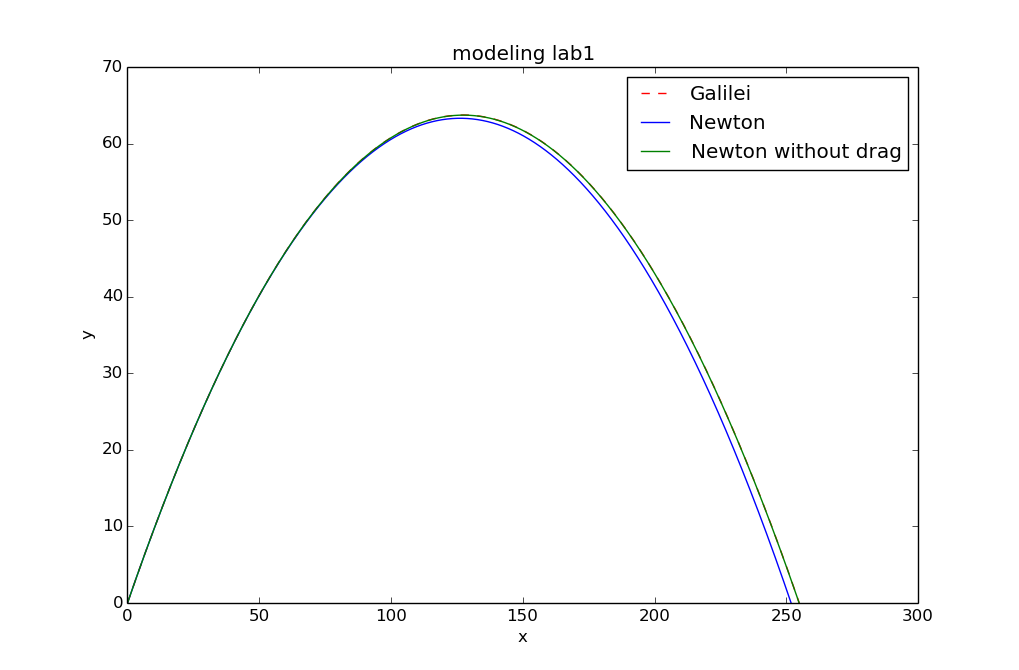
\includegraphics[scale=0.65]{figure_1.png}
        \caption{Траектории полёта снарядов для различных моделей}
        \label{pic:figure}
    \end{figure}

    \begin{figure}[h!]
        \centering
        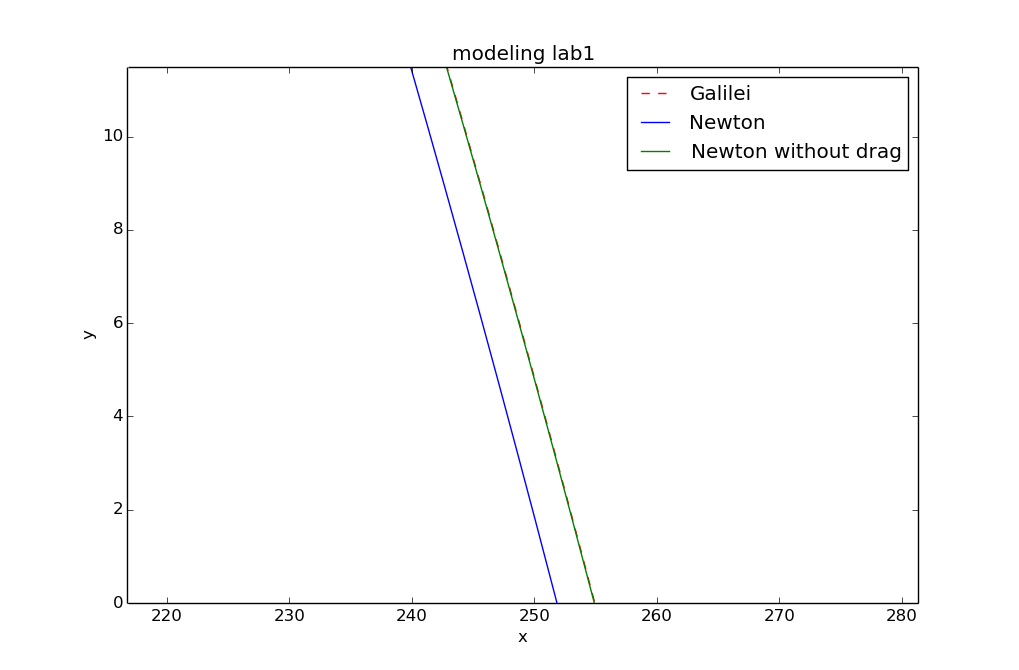
\includegraphics[scale=0.65]{figure_1_zoom.png}
        \caption{Траектории полёта снарядов для различных моделей}
        \label{pic:figure_zoom}
    \end{figure}

\section{Анализ результатов}
    Результаты обоих моделей без учёта сопротивления воздуха совпали, что говорит о корректности этих моделей. Как и ожидалось, сопротивление воздуха сократило дальность полёта снаряда.

\end{document}